Das folgende Diagramm \vref{ausfuehrungssicht} zeigt das Laufzeitverhalten der Software.
Auf der einen Seite haben wir den mobilen Zugang, auf dem die Android App als Prozess läuft. Die App selbst verwendet die Module \texttt{net.requests}, \texttt{net.responses}, \texttt{net}, \texttt{mygdx.game} und \texttt{mygdx.net}. Von diesem mobilem Zugang kann eine TCP/IP-Verbindung zu dem Server aufgebaut werden. Dabei gibt es mehrere Verbindungen zu immer nur einem Server, daher die Multiplizitäten \texttt{*} und \texttt{1}.

Auf der anderen Seite nimmt nun der Server die TCP/IP-Verbindungen an. Er ist gleichzeitig Server und Datenbankserver. Der Server verwendet die Module \texttt{net.requests}, \texttt{net.responses}, \texttt{net}, \texttt{server.persistence} und \texttt{server}.

Das komplette System läuft mit zwei Prozessen: Einmal mit der Android App und dem anderen Prozess Server. Prinzipiell gibt es unendlich viele mobile Zugänge bzw. App-Prozesse, die auf einen Server zugreifen.

\begin{figure} [H] 
\caption{Ausführungssicht} 
	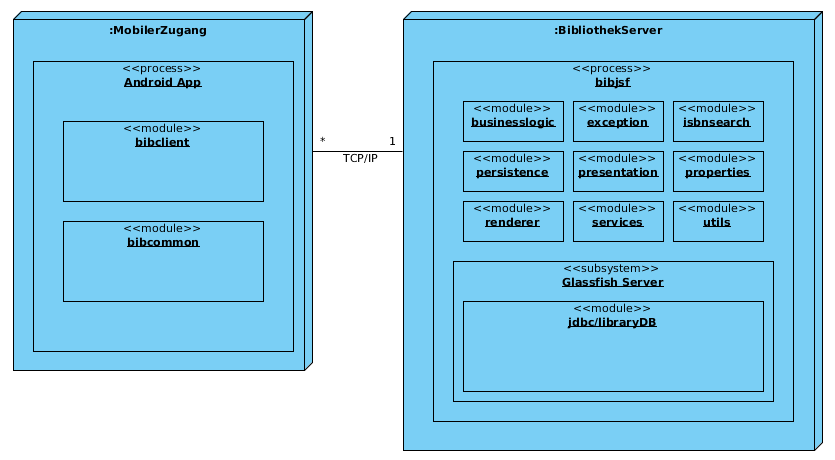
\includegraphics[width=1\textwidth]{Diagramme/ausfuehrungssicht.png} 
	\label{ausfuehrungssicht} 
\end{figure}
